We present the results of our abstraction-based method for surveillance strategy synthesis on two case studies. We use slugs, a generalized reactive synthesis tool detailed in \cite{EhlersR16}. Simulations were run on a Intel i5-5300U 2.30 GHz CPU with 8 Gb of ram. 

\subsection{Liveness surveillance specification + task specification}
Figure~\ref{fig:case1} shows a gridworld divided into  'rooms'. The surveillance objective requires the agent to infinitely often know precisely the location of the target (either see it, or have a belief consisting of one cell). Additionally, it has to perform the task of patrolling (visiting infinitely often) the green 'goal' cell. Formally, the specification is $\LTLglobally\LTLfinally p_1 \wedge \LTLglobally\LTLfinally \mathit{goal}$. 


\begin{figure}
\centering
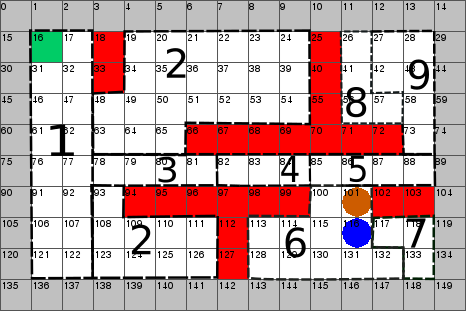
\includegraphics[scale=0.3]{text970.png}\caption{Gridworld with a computed partition of size $9$.}\label{fig:case1}
\vspace{-.5cm}
\end{figure}

%\begin{table}[h!]
%\begin{tabular}{c|c|c|c}
%& Not refined & Partially refined & Fully refined \\ \hline \hline
%Number of states & 104 & 616 & $2\times10^{31}$
%\end{tabular}
%\end{table}

Starting with an abstract game with 104 states generated by a partition with two elements, our refinement algorithm terminates after 5 iterations (with total running time of 821 s). The resulting partition $\mathcal{Q} = \{Q_1,...,Q_9 \}$ has $9$ elements shown as the numbered regions in Figure~\ref{fig:case1}. Thus, the final refined abstract game has $616$ abstract states ($2^9$ abstract belief states). In contrast, the belief-set game structure would have $2^{104}$ states, which is state-space size that state-of-the-art synthesis tools are not capable of handling.


%The refinement algorithm terminates after 5 iterations to produce the abstract partition  corresponding to the numbered sets in figure . There are 9 belief states which results in an additional $2^9 = 512$ states to the full observation game which is far lower than the full reduction which will be a power set of all 104 states.

A video simulation can be found at \url{http://goo.gl/YkFuxr}. Note the behaviour of the agent visiting the goal and then searching for the target. This will contrast with the behaviour under safety surveillance objectives which we look at next.

\subsection{Safety surveillance specification + task specification}
\begin{figure}
\centering
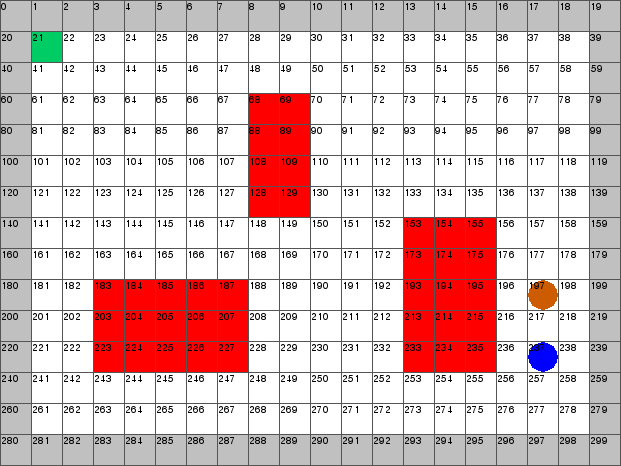
\includegraphics[scale=0.2]{case2.png}\caption{Gridworld representing an outdoor environment.}\label{fig:case2}
\vspace{-.5cm}
\end{figure}
Figure~\ref{fig:case2} depicts a gridworld of an 'outdoor' environment where the red blocks model buildings. 
In this setting, we enforce the safety surveillance objective $\square p_{30}$ in addition to infinitely often reaching the green cell. The formal specification is $\LTLglobally\LTLfinally p_{30} \wedge \LTLglobally\LTLfinally \mathit{goal}$. 
We used an abstraction generated by a partition of size 6, which was sufficiently precise to compute a surveillance strategy in 210 s. This demonstrates that even for larger grids, a coarse abstraction can be sufficient. Again, note that the precise belief-set game would have in the order of $2^{200}$ states.
 
We simulated the environment and the synthesized surveillance strategy for the agent in ROS. A video of the simulation can be found at \url{http://goo.gl/LyC1gQ}. Note the qualitative difference in behaviour compared to the previous example. In the case of liveness surveillance, the agent had more leeway to completely lose the target in order to reach its goal location, even though the requirement of reducing the size of the belief to $1$ is quite strict. Here, on the other hand, the safety surveillance objective, even with a large threshold of $30$, forces the agent to follow the target more closely, in order to prevent its belief from getting too large. The algorithm thus provides the ability to obtain qualitatively different behaviour as necessary for specific applications by combining these objective types. 

%\Suda{Not sure if we should keep this next part}
%\subsection{Discussion of behaviour}
%The difference in the behaviour in the case studies highlights the different use cases of the surveillance objectives. In more indoor settings or structured environments, a liveness surveillance objective is feasible as the agent can more easily search and find the target even if the belief grows very large. However, in outdoor environments this is harder to accomplish as the target has more room to hide. 